Models such as Stable Diffusion are developed by training on extensive datasets, enabling them to grasp intricate details about a wide range of concepts. Introducing a new concept, such as incorporating images of your dog, to generate further images in various styles, is an intriguing and essential capability for numerous tasks. This includes editing images or transferring the style of your image to create a new one. The ability to seamlessly add personal or unique elements into the model's database not only enhances its versatility but also opens up new avenues for creativity and customization. This process of enriching the model with additional, specific data points allows for a more tailored and personalized user experience, making it invaluable for tasks ranging from personal projects to professional endeavors that require a high degree of customization and artistic flair.

\subsection{Learning}

Incorporating new concepts into generative models, particularly diffusion models like Stable Diffusion, represents a significant stride toward enhancing the versatility and personalization capabilities of these models in image generation. This advancement is primarily facilitated through two distinct methodologies: embedding-based learning and full model training.

\subsection{Embedding-based Learning}
Embedding-based learning focuses on integrating new concepts into the model through specialized embeddings, which are pivotal in teaching the model to recognize and generate images based on newly incorporated ideas. Textual Inversion, for instance, is at the forefront of this approach, specializing in learning textual embeddings for a new concept. This technique enables the model to understand and produce images that embody unique or personal subjects, essentially customizing the model to grasp novel ideas beyond its initial training data \cite{textualInversion}. Complementing this, ReVersion shifts the emphasis toward learning embeddings that capture the relational dynamics between concepts. It delves into understanding the interconnections between new and existing concepts within the model, thus facilitating a more nuanced and context-aware integration of new ideas \cite{reVersion}. This embedding-centric approach not only enhances the model's generative capabilities but also ensures that the integration of new concepts is done in a manner that respects the nuanced relationships between different ideas, enabling more cohesive and contextually relevant outputs.


\begin{figure}[h!]
    \centering
    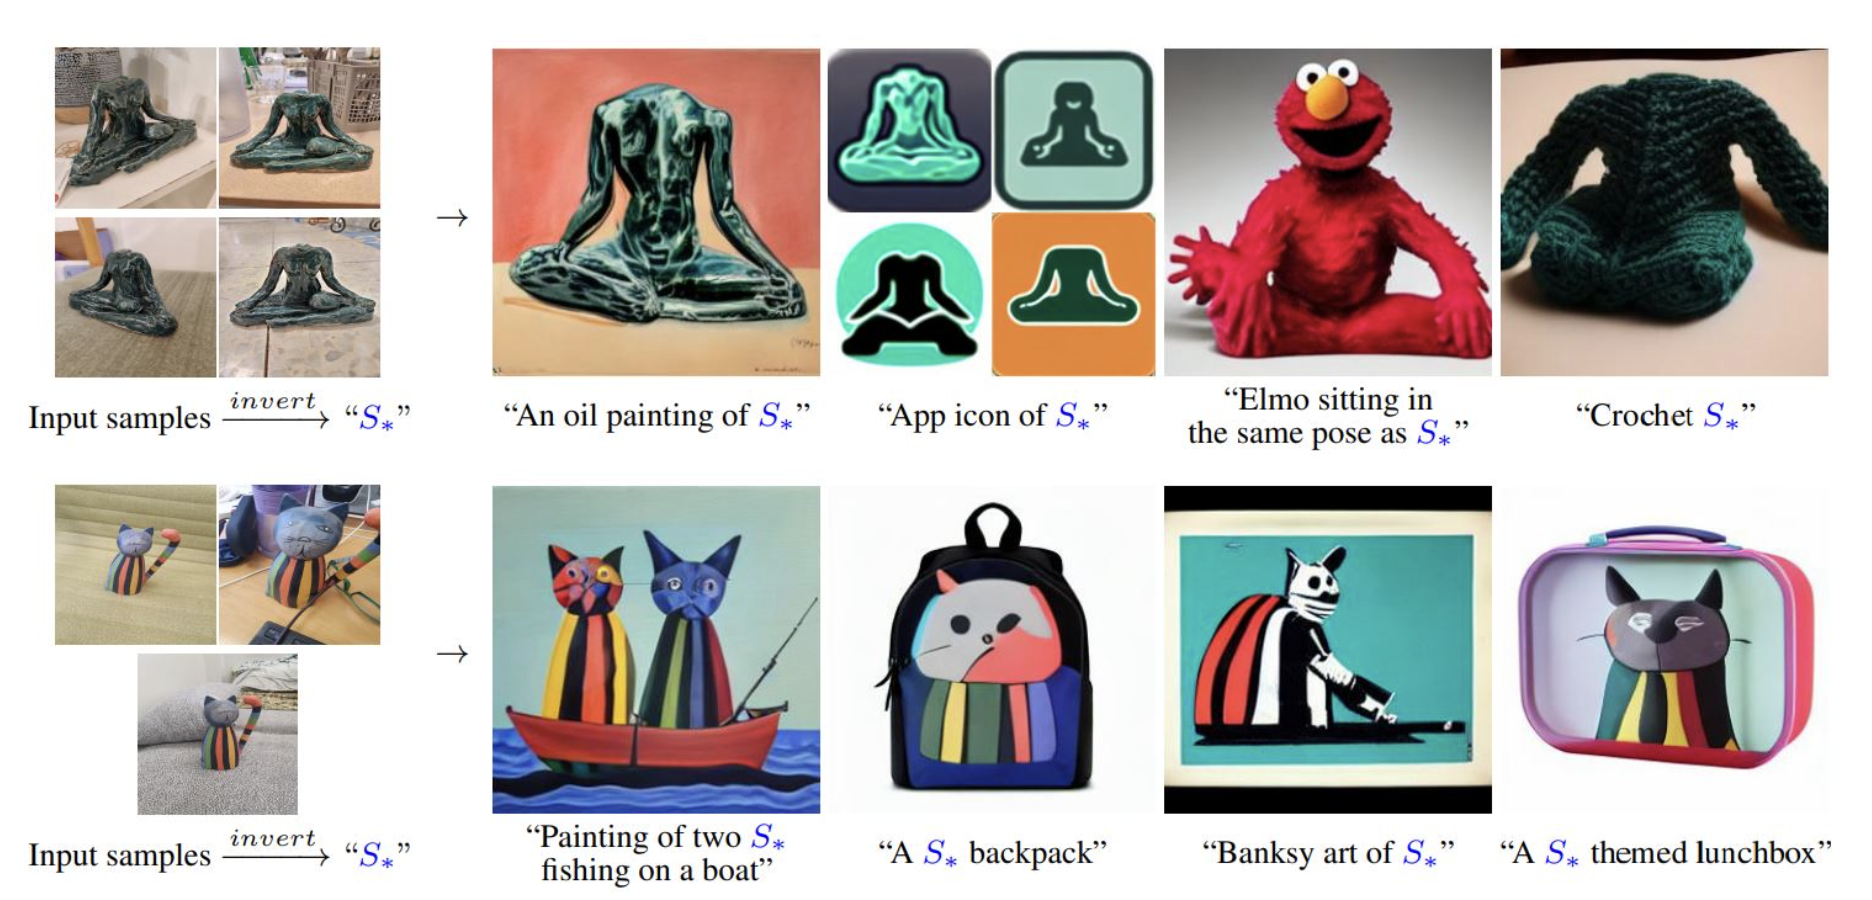
\includegraphics[width=\textwidth]{images/ti.png}
    \caption{Textual Inversion Results \cite{textualinversion2022}}
\end{figure}


\subsection{Full Model Training}
On the other side of the spectrum, full model training approaches such as Dreambooth push the boundaries by employing autogenous, class-specific prior preservation. This technique fine-tunes the entire model to adeptly generate images of a specific subject in various contexts, thereby broadening the model's versatility and adaptive capabilities \cite{dreambooth}. Similarly, Custom Diffusion updates the model by fine-tuning a selective set of weights, specifically targeting the key and value mappings in the cross-attention layers. This method underscores a targeted and efficient means of updating the model, ensuring that new concepts are seamlessly woven into the model's fabric without extensive retraining \cite{customDiffusion}. Furthermore, SINE reimagines model modification through classifier-free guidance (CFG) adjustments, enhancing the model's fidelity to desired outputs in the absence of explicit class labels, thus offering a robust and flexible framework for concept introduction \cite{sine}. Lastly, Break-A-Scene introduces a novel paradigm by enabling the learning of multiple concepts from a singular image, deviating from the conventional one-concept-per-multiple-images approach. This strategy showcases an efficient pathway to enrich the model's comprehension and creative scope \cite{breakAScene}. Through these full model training techniques, the landscape of generative modeling is witnessing a paradigm shift towards more dynamic, adaptive, and personalized image generation, promising a future where models can more accurately reflect the diversity and specificity of human imagination.




The convergence of these methodologies underlines a pivotal evolution in the development of diffusion models, marking a significant leap toward creating more adaptive, personalized, and context-aware generative models.









\begin{equation} \label{eq:1}
    \mathbb{E}_{x,c,e,\varepsilon,t} \left[ w_t \left\| \mathcal{X}_\theta (\alpha_t X + \sigma_t \varepsilon, c) - X \right\|^2 \right] 
    + \lambda w_t' \left\| \mathcal{X}_\theta (\alpha_t' X_{pr} + \sigma_t' \varepsilon', c_{pr}) - X_{pr} \right\|^2,
    \end{equation}



\begin{figure}[H]
    \centering
    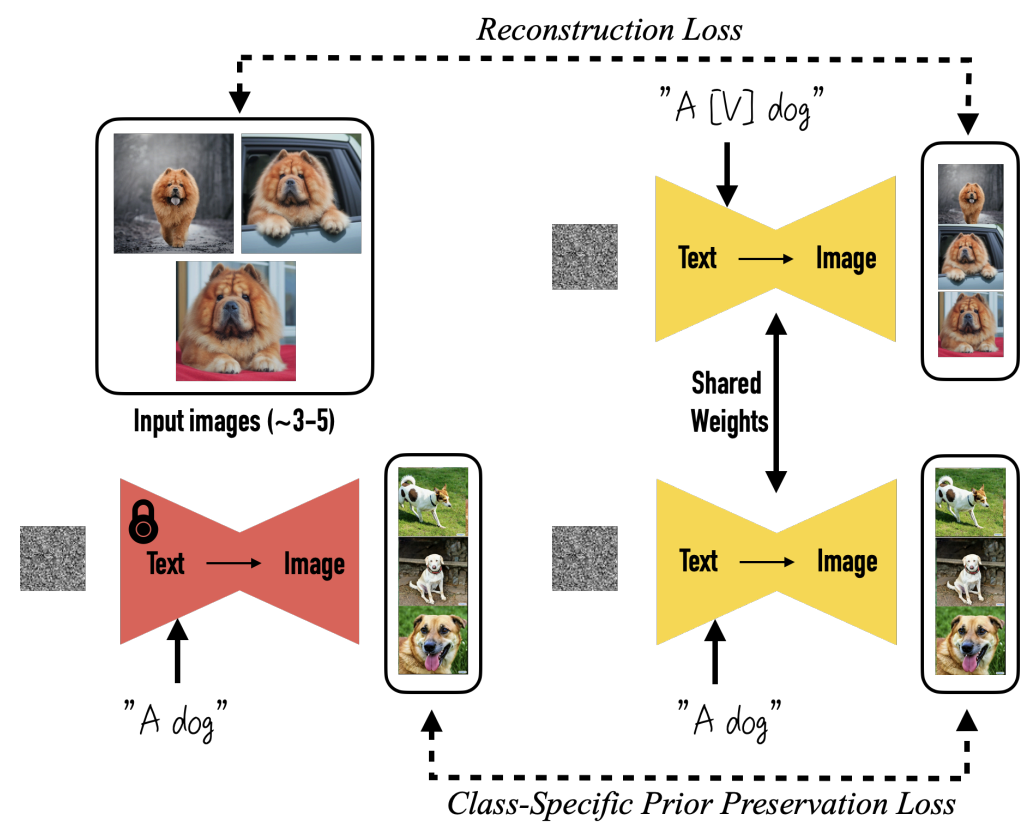
\includegraphics[width=0.55\textwidth]{images/dreambooth_training.png}
    \caption{Finetuning Dreambooth: Fine-tuning. Given $\sim 3-5$ images of a subject we finetune a text-to-image diffusion model with the input images paired
    with a text prompt containing a unique identifier and the name of
    the class the subject belongs to (e.g., "A [V] dog"), in parallel, we
    apply a class-specific prior preservation loss, which leverages the
    semantic prior that the model has on the class and encourages it to
    generate diverse instances belong to the subject's class using the class name in a text prompt (e.g., "A dog"). \cite*{dreambooth}}
\end{figure}
    

\begin{figure}[H]
    \centering
    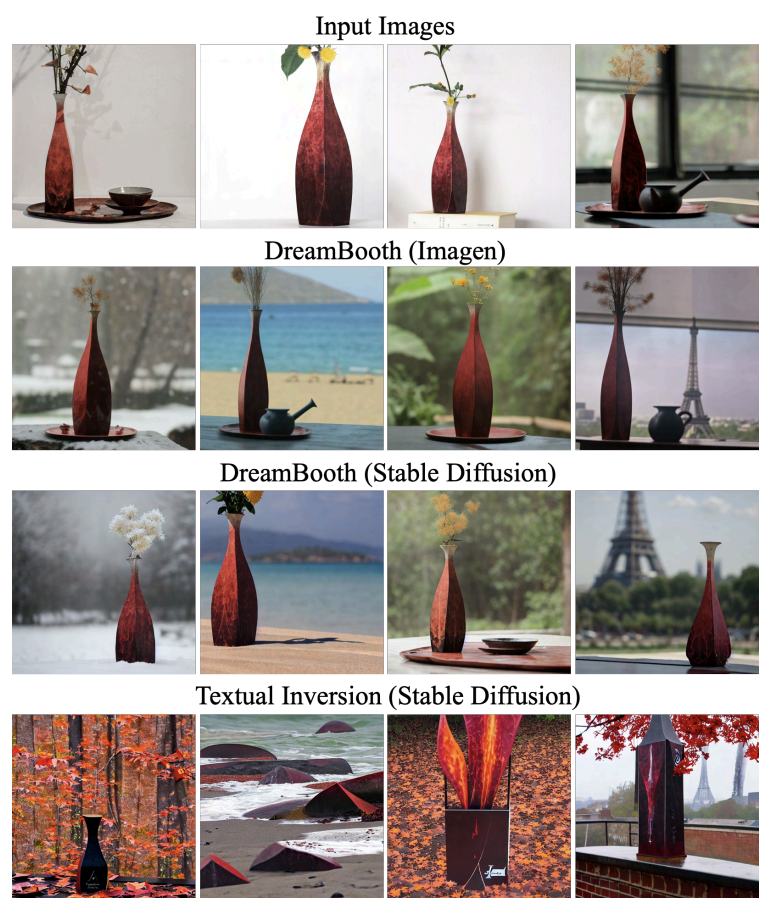
\includegraphics[width=0.4\textwidth]{images/dreambooth_ti_comp.png}
    \caption{Comparisons with Textual Inversion [20] Given 4
    input images (top row), we compare: DreamBooth Imagen (2nd
    row), DreamBooth Stable Diffusion (3rd row), Textual Inversion
    (bottom row). Output images were created with the following
    prompts (left to right): “a [V] vase in the snow”, “a [V] vase on
    the beach”, “a [V] vase in the jungle”, “a [V] vase with the Eiffel
    Tower in the background”. DreamBooth is stronger in both subject
    and prompt fidelity. \cite*{dreambooth}}
\end{figure}

\begin{table}[h!]
    \centering
    \begin{tabular}{ | m{5em} | m{5cm}| m{8cm} | m{2cm} | }
    \hline
    \textbf{Name} & \textbf{Tags} & \textbf{Text} & \textbf{Citations} \\
    \hline
    Textual Inversion & Embeddings & Learns textual embedding for new concept &  \\
    \hline
    Dreambooth & Full model \newline new loss & Trains full model using autogenous, class-specific prior preservation loss & \cite*{dreambooth}  \\
    \hline
    Custom Diffusion & Learns Attention KV & A small subset of model weights, namely the key and value mapping from text to latent features in the cross-attention layers. Fine-tuning these is sufficient to update the model with the new concept & \cite{customDiffusion} \\
    \hline
    ReVersion: & Embeddings & Learns embedding to learn relation instead of feature of image & \cite{reVersion} \\
    \hline
    SINE & Modifies CFG & Model-based classifier-free guidance & \cite{sine}\\
    \hline
    Break-A-Scene & Learning multiple concept & Learning multiple concepts using single image instead of learning one concept using multiple images & \\
    \hline
    \end{tabular}
    \caption{Contribution of different concept learning methods}
\end{table}
    